\documentclass[11pt, oneside]{article} 
\usepackage{geometry}
\geometry{letterpaper} 
\usepackage{graphicx}
	
\usepackage{amssymb}
\usepackage{amsmath}
\usepackage{parskip}
\usepackage{color}
\usepackage{hyperref}

\graphicspath{{/Users/telliott_admin/Dropbox/Tex/png/}}
% \begin{center} 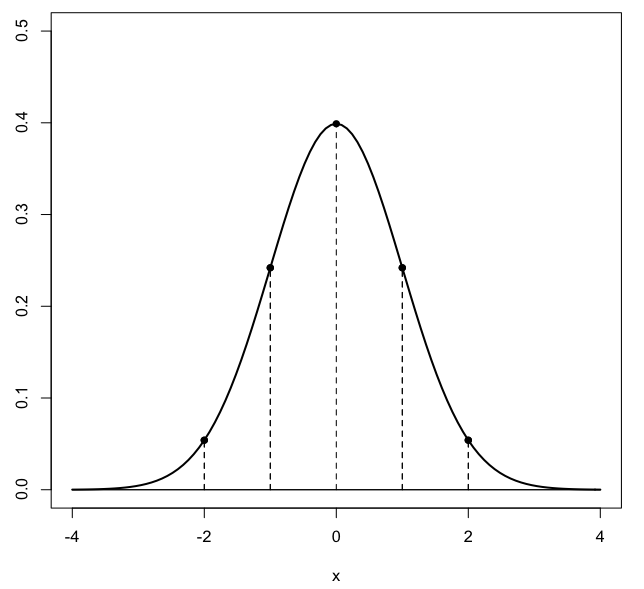
\includegraphics [scale=0.4] {gauss3.png} \end{center}

\title{Feynman's Dots}
\date{}

\begin{document}
\maketitle
\Large

Richard Feynman gave a famous series of talks at Cornell in 1964 that were videotaped and transcribed into a book.  Bill Gates later purchased them and put them on the web, unfortunately with some Microsoft DRM.  

Still, I have the book, called \emph{The Character of Physical Law}.  This argument is from Chapter 2, \emph{The Relation of Mathematics to Physics}.

It depends on a tiny bit of calculus.  Specifically, it uses the product rule for differentiation, plus the fact that the product rule is valid for vector cross products.  Here is a short write-up on the subject, from my book \emph{Best of Calculus}.

\subsection*{time-derivative of products}
To take the derivative with respect to the parameter (such as time), we just go through each component of a vector one at a time:
\[ \mathbf{r} = \langle x, y, z \rangle \]
\[ \frac{d \mathbf{r}}{dt} =  \langle \frac{dx}{dt}, \frac{dy}{dt}, \frac{dz}{dt} \rangle \]

The question arises, what about products?  Is there a product rule for vectors?  Here's an example
\[ \frac{d}{dt} \ \mathbf{r} \cdot \mathbf{v} \]
It turns out that there is.
\[ \frac{d}{dt} \ \mathbf{r} \cdot \mathbf{v} = \frac{d \mathbf{r}}{dt} \cdot \mathbf{v} + \mathbf{r} \cdot \frac{d \mathbf{v}}{dt}  \]
The reason is that the individual components of the dot product are simple functions of $t$, and our rule is to differentiate one component at a time.

Let's use Newton's dot notation for $d/dt$:
\[ \mathbf{r} = \langle x, y, z\rangle \]
\[ \mathbf{\dot{r}} = \mathbf{v} = \langle \dot{x}, \dot{y}, \dot{z} \rangle \]
\[ \mathbf{r} \cdot \mathbf{\dot{r}}  = x \dot{x} + y \dot{y} + z \dot{z} \]
The derivative is
\[ \frac{d}{dt} \mathbf{r} \cdot \mathbf{\dot{r}}  = \frac{d}{dt} ( x \dot{x} + y \dot{y} + z \dot{z} ) \]
\[ = \dot{x} \dot{x} + x \ddot{x} + \dot{y} \dot{y} + y \ddot{y} + \dot{z} \dot{z} + z \ddot{z}  \]
\[ = \dot{x} \dot{x} + \dot{y} \dot{y} + \dot{z} \dot{z} + x \ddot{x}  + y \ddot{y} + z \ddot{z}  \]
\[ =  \mathbf{\dot{r}} \cdot \mathbf{\dot{r}} +  \mathbf{r} \cdot \mathbf{\ddot{r}} \]

The same is true of the cross-product.  The torque is $\mathbf{F} \times \mathbf{r}$  Let's take the derivative:
\[ \frac{d}{dt} \ [ \ \mathbf{F} \times \mathbf{r} \ ] \ = \]
Let's write $\mathbf{F} = \langle M,N,P \rangle$, then the cross-product gives a vector with components
\[ \ [ \ N z - P y \ ] \ \mathbf{\hat{i}} + \ [ \ P x - M z \ ] \ \mathbf{\hat{j}} + \ [ \ M y - N x \ ] \ \mathbf{\hat{k}} \]
where all of $M,N,P$ and $x,y,z$ are \emph{functions} of time.

The time derivative is obtained by the product rule.  Again, I will use dots, and here we separate the components onto different lines:
\[ \ [ \ \dot{N} z + N \dot{z} - \dot{P} y - P \dot{y} \ ] \ \mathbf{\hat{i}} + \]
\[ + \  [ \ \dot{P} x + P \dot{x} - \dot{M} z - M \dot{z} \ ] \ \mathbf{\hat{j}} + \]
\[ +  \ [ \ \dot{M} y + M \dot{y} - \dot{N} x - N \dot{x} \ ] \ \mathbf{\hat{k}} \]

but this is just two different cross-products added together.  The first one is
\[ \ [ \ \dot{N} z - \dot{P} y \ ] \ \mathbf{\hat{i}} + \  [ \ \dot{P} x - \dot{M} z \ ] \ \mathbf{\hat{j}} +  \ [ \ \dot{M} y - \dot{N} x \ ] \ \mathbf{\hat{k}} \]
\[ = \mathbf{\dot{F}} \times \mathbf{r} \]

and the second is:
\[ \ [ \  N \dot{z}  - P \dot{y} \ ] \ \mathbf{\hat{i}} + \  [ \ P \dot{x} - M \dot{z} \ ] \ \mathbf{\hat{j}} +  \ [ \ M \dot{y} - N \dot{x} \ ] \ \mathbf{\hat{k}} \]
\[ = \mathbf{F} \times \mathbf{\dot{r}} \]

Putting it all together
\[ \frac{d}{dt} \ [ \ \mathbf{F} \times \mathbf{r} \ ] \ = \mathbf{\dot{F}} \times \mathbf{r} + \mathbf{F} \times \mathbf{\dot{r}} \]

The product rule for differentiation holds for both the dot product and the cross-product.

\subsection*{Do the dots}

The rule is that if we have two vectors $\mathbf{a}$ and $\mathbf{b}$ which are changing (i.e. they are functions of time), then
\[ \frac{d}{dt} \ (\mathbf{a} \times \mathbf{b}) = \frac{d\mathbf{a}}{dt} \times \mathbf{b} + \mathbf{a}  \times \frac{d\mathbf{b}}{dt}    \]
In our application the two vectors are the position vector of the planet with respect to the sun, $\mathbf{r}$, and the time-derivative of that vector.
\[ \frac{d\mathbf{r}}{dt} = \mathbf{v} \]
Or, using Newton's dot notation for the time-derivative:
\[ \mathbf{v} = \dot{\mathbf{r}} \]

We are interested in the area of the triangle formed by the vectors $\mathbf{r}$ and $\dot{\mathbf{r}}$ over a small interval of time.  The area swept out is constant, as Newton showed, and we will prove again here.

A nice feature of the vector cross-product is that it provides (twice) this area.  Namely
\[ A =  \mathbf{r} \times \dot{\mathbf{r}} = |\mathbf{r}| |\dot{\mathbf{r}}| \sin \theta   \]
where $\theta$ is the angle between $\mathbf{r}$ and $\dot{\mathbf{r}}$, and $A$ is the little bit of additional area.

Our hypothesis is that $A$ is the same no matter where the planet is in its orbit.  Another way to say the same thing is that A doesn't change with time
\[ \frac{d}{dt} \ A = \dot A = 0 \]
Now 
\[ A = \mathbf{r} \times \dot{\mathbf{r}} \]
and we want to compute $\dot A$.  Using the product rule it's easy.
\[ \dot A = \frac{d}{dt} \ (\mathbf{r} \times \dot{\mathbf{r}}) \]
\[ \dot A = \dot{\mathbf{r}} \times \dot{\mathbf{r}} \ + \ \mathbf{r} \times \ddot{\mathbf{r}} \]
As Feynman says: it's just playing with dots.  So let's look at those two terms.  Another nice fact about the cross-product is that if the two vectors point in the same direction, then the cross-product is zero.

Any vector points in the same direction as itself, so the first term is certainly zero.  
\[ \dot{\mathbf{r}} \times \dot{\mathbf{r}} \ = 0 \]
Next, recall that the second derivative with respect to time of the position is the acceleration vector.  According to Newton's second law, the force of gravity points toward the sun, radially.  

But of course the position vector also points out radially from the sun.  $\mathbf{r}$ and $\ddot{\mathbf{r}}$ are in the same direction (the opposite direction \emph{is} the same direction, multiplied by $-1$), so the cross-product is again zero.
\[ \mathbf{r} \times \ddot{\mathbf{r}} \ = 0 \]
So that means the whole thing is zero.
\[ \dot A = \dot{\mathbf{r}} \times \dot{\mathbf{r}} \ + \ \mathbf{r} \times \ddot{\mathbf{r}} = 0 + 0 = 0  \]
We have shown that the area is constant, which is Kepler's second law.  By the way, the invariant quantity 
\[ \mathbf{r} \times \mathbf{v} = \mathbf{r} \times \dot{\mathbf{r}} \]
(times the mass) is the angular momentum, and the lack of change is the principle of the conservation of angular momentum.

Note:  in this section we have followed Feynman (who was trying to make the argument as simple as possible).  He called the area swept out in a small interval of time $A$ and showed that $\dot{A} = 0$.  

It would be more appropriate it to call it $dA/dt$, the instantaneous rate of change of the area.  Then the quantity that is equal to zero is the time-derivative of \emph{that}, namely:  $d^2A/dt^2$.

\end{document}  